% This is "sig-alternate.tex" V2.1 April 2013
% This file should be compiled with V2.5 of "sig-alternate.cls" May 2012
%
% This example file demonstrates the use of the 'sig-alternate.cls'
% V2.5 LaTeX2e document class file. It is for those submitting
% articles to ACM Conference Proceedings WHO DO NOT WISH TO
% STRICTLY ADHERE TO THE SIGS (PUBS-BOARD-ENDORSED) STYLE.
% The 'sig-alternate.cls' file will produce a similar-looking,
% albeit, 'tighter' paper resulting in, invariably, fewer pages.
%
% ----------------------------------------------------------------------------------------------------------------
% This .tex file (and associated .cls V2.5) produces:
%       1) The Permission Statement
%       2) The Conference (location) Info information
%       3) The Copyright Line with ACM data
%       4) NO page numbers
%
% as against the acm_proc_article-sp.cls file which
% DOES NOT produce 1) thru' 3) above.
%
% Using 'sig-alternate.cls' you have control, however, from within
% the source .tex file, over both the CopyrightYear
% (defaulted to 200X) and the ACM Copyright Data
% (defaulted to X-XXXXX-XX-X/XX/XX).
% e.g.
% \CopyrightYear{2007} will cause 2007 to appear in the copyright line.
% \crdata{0-12345-67-8/90/12} will cause 0-12345-67-8/90/12 to appear in the copyright line.
%
% ---------------------------------------------------------------------------------------------------------------
% This .tex source is an example which *does* use
% the .bib file (from which the .bbl file % is produced).
% REMEMBER HOWEVER: After having produced the .bbl file,
% and prior to final submission, you *NEED* to 'insert'
% your .bbl file into your source .tex file so as to provide
% ONE 'self-contained' source file.
%
% ================= IF YOU HAVE QUESTIONS =======================
% Questions regarding the SIGS styles, SIGS policies and
% procedures, Conferences etc. should be sent to
% Adrienne Griscti (griscti@acm.org)
%
% Technical questions _only_ to
% Gerald Murray (murray@hq.acm.org)
% ===============================================================
%
% For tracking purposes - this is V2.0 - May 2012
\documentclass{sig-alternate-05-2015}

\usepackage{comment}    % For block comments
\usepackage{cite}       % For group citations
\usepackage{color}      % For warnings and draft notations
\usepackage{float}

\graphicspath{ {figures/rGraphs/} }

\begin{document}

% Copyright
\setcopyright{acmcopyright}
%\setcopyright{acmlicensed}
%\setcopyright{rightsretained}
%\setcopyright{usgov}
%\setcopyright{usgovmixed}
%\setcopyright{cagov}
%\setcopyright{cagovmixed}


% DOI
\doi{}

% ISBN
\isbn{}

%Conference
%\conferenceinfo{PLDI '13}{June 16--19, 2013, Seattle, WA, USA}
%\acmPrice{\$15,000}

%
% --- Author Metadata here ---
%\conferenceinfo{WOODSTOCK}{'97 El Paso, Texas USA}
%\CopyrightYear{2016} % Allows default copyright year (20XX) to be over-ridden - IF NEED BE.
%\crdata{0-12345-67-8/90/01}  % Allows default copyright data (0-89791-88-6/97/05) to be over-ridden - IF NEED BE.
% --- End of Author Metadata ---

\title{Software Developers and Computers as Social Actors}
%\subtitle{A Nass Replication}
%

\numberofauthors{1} %  in this sample file, there are a *total*
% of EIGHT authors. SIX appear on the 'first-page' (for formatting
% reasons) and the remaining two appear in the \additionalauthors section.
%
\author{Prairie Rose Goodwin \qquad Adam Marrs \qquad Matthew Neal \qquad Shaown Sarker\\ \\ \affaddr{Department of Computer Science}\\ \affaddr{North Carolina State University}\\ \email{\normalsize \{prgoodwi,acmarrs,mneal,ssarker\}@ncsu.edu}\\}


\maketitle
\begin{abstract}
Surveys are a commonly used for assessment purposes in software engineering, but developers are rarely aware of biases inherent in computer-based evaluations.  In 1999, Nass et al. conducted a series of studies which indicated that people exhibit social biases towards computers. We conducted a theoretical replication of Nass's original experiment to evaluate these effects in software engineers. Our results suggest that a developers' intricate knowledge of computers may diminish or eliminate the behaviors observed in previous experiments with different demographics. Furthermore, our experimental design can inform future survey-based experiments that aim to compare the behaviors of software engineers and non-software engineers.

\begin{comment}In 1999, Nass et al. conducted a series of studies to establish the presence of normative-response bias and interviewer-based bias in human responses to a computer interviewer agent. During the time since the study, computers have become prevalent in society and are an integral component of both personal and professional life. In our work, we conduct a theoretical replication of the study by Nass and colleagues to verify whether the results of the study still holds in today's more technologically savvy society. We also study the bias in detail among software developers who maintain a collaborative relationship with their computers by comparing their responses with non-software developer participants. Our findings show that human social biases regarding interview are still present in responses to computers, and software developers also demonstrate this bias despite the contrary perception that they should not hold such biases given their intricate knowledge of the computer as the interviewer.
\end{comment}

\end{abstract}

%
% The code below should be generated by the tool at
% http://dl.acm.org/ccs.cfm
% Please copy and paste the code instead of the example below. 
%

\begin{CCSXML}
<ccs2012>
<concept>
<concept_id>10003120.10003121</concept_id>
<concept_desc>Human-centered computing~Human computer interaction (HCI)</concept_desc>
<concept_significance>500</concept_significance>
</concept>
</ccs2012>
\end{CCSXML}


\ccsdesc[500]{Human-centered computing~Human computer interaction (HCI)}

%
%  Use this command to print the description
%
\begin{comment}
\printccsdesc
\end{comment}

\keywords{software engineering; computers as social actors}

\section{Introduction}
In research interviews, honest and forthcoming answers are essential to the process. Interviews are plagued by biases inherent in social interactions. Such biases include the normative-response bias (people not wanting to admit to answers that are counter to the perceived norm), interviewer-based bias (people answering based on the perceived preference of the interviewer), and politeness norms (people modifying answers to avoid offending). Computer systems were introduced to mitigate these known social biases by providing anonymity and an emotionless interviewer.  Since everyone is aware that computers do not have feelings, it was assumed that the phenomenon would not transfer to human computer interaction. 

Through a series of studies, Nass et al. documented how individuals anthropomorphize technology and exhibit attitudes previously thought to be reserved for person to person interaction\cite{nass1999people}\cite{reeves1996people}.  In the first study, participants interacted with an intelligent tutoring system and were asked to evaluate the system in one of three conditions: 1) evaluating the system on the same physical computer, 2) evaluating the system on a different but identical computer, or 3) evaluating the system with a pen-and-paper questionnaire. Their results showed that participants rated the intelligent tutoring system on the same computer more positively and more homogeneously than in the other conditions. The results suggested that humans unintentionally, unknowingly apply social rules to computer systems.  


The way people interact with computers has changed significantly since the study was published  in 1999.  Computers are now an integral part of both personal and professional life, and users often form strong bonds with their personal devices.  Software developers are more aware of the inanimate nature of machines, but they likely spend more time in front of a computer than those in other professions. Our study is a theoretical replication that measures the effects of social biases in software engineers.  Moreover, we want to test whether using a personal machine introduces a stronger social bias than public computers.Therefore, we designed an experiment to answer the following research questions:\\

\noindent \textbf{\emph{Research Question 1:}} do software developers exhibit the social bias phenomena identified in previous studies?\\

\noindent \textbf{\emph{Research Question 2:}} does a software developer's familiarity with a computing environment affect the social bias phenomena?\\

\begin{comment}
\begin{enumerate}
    \item{Does programming experience affect the social bias phenomena?}
    \item{Does a software developer's familiarity with a computer affect the social bias phenomena?} 
\end{enumerate}
\end{comment}

We recreated Nass's intelligent tutor using the details found in the original paper. Our experiment has two independent variables to test the two research questions:
\begin{enumerate}
    \item{\emph{Evaluation method:} Participants either used one computer for the entire experiment, or they completed the Evaluation Session on an identical pen-and-paper questionnaire.}
    \item {\textit{Computing environment}: Participants either used their personal laptops or a public computer in a computer lab.}
\end{enumerate}


\begin{comment}
\begin{enumerate}
    \item {\textit{Evaluation method}: Participants either used one computer for the entire experiment, or they completed the final evaluation on an identical pen-and-paper questionnaire.}
    \item {\textit{Computing environment}: Participants either used personal laptops or a public computer in a computer lab.}
\end{enumerate}
\end{comment}

\section{Related Work}
Previous research demonstrates that computers are often treated as social entities despite their inanimate nature. Some studies have focused on the human application of social norms and expectations to computers in a seamless manner. In addition to the original study, Nass et al. performed a series of follow-up experiments that suggest that social stereotypes attributed to gender, ethnicity, and group loyalty, along with deeply ingrained social habits and behaviors like, reciprocity and reciprocal self-disclosure, are extended to computers when interacting with them~\cite{Nass2000machines,nass1999people}. Moreover, this behavior is not only limited to computers, human users anthropomorphize other technological mediums like television~\cite{reeves1996people}.

\begin{comment}
The authors concluded that doing the evaluation on a different computer was experimentally equivalent to doing the evaluation with pen-and-paper.  \footnote{A more recent, but unpublished replication study found that using a different computer resulted in the same effect as using the same computer\cite{gownivaripalli}.}  
\end{comment}


These findings engendered a number of studies that extended on this implication by replicating, validating, and exploring the possible factors behind these kind of responses. The existing Computers as Social Actors (CASA) studies featured an implicit bias - although the studies were conducted with participants exclusively from the United States, the findings were generalized to all cultures. Katagiri and colleagues performed a comprehensive study to determine whether social rules derived from different cultures affect human users responses to computers by observing participants from the United States and Japan~\cite{katagiri2001cross}. Furthermore, researchers studied the existence of computers as social entities to better understand racial biases in interviews\cite{krysan2003race}, how the quality of interaction affects expressive systems \cite{vidyarthi2011sympathetic}, and even how to leverage social cues to more effectively sell products online \cite{wang2007can}. In contrast, our work explores the effect of viewing computers as a human-like social entity on the very specific demographic of software developers and attempts to determine the level of politeness software developers exhibit toward their machines.

Software developers maintain a collaborative environment with their computers to complete their tasks. Given software developers' advanced understanding of how computers work, one would expect the attribution of social qualities to computers to be minimal or not present.  This type of attribution would be expected, if the the sociability of a computer system is modified by the quality of an individual's mental model of a computer system. Research has shown that human-computer team performance is higher when human users have accurate mental models~\cite{wilkison2007effects}. Further studies by Bickmore and Picard have documented the long-term relation establishment and maintenance between a human-computer team by observing that human users of a relational computer agent did not only respect, trust, and like the agent, but also wanted to continue working with the agent even after the end of the study~\cite{Bickmore:2005:EML:1067860.1067867}. In this paper, we investigate whether a long term relationship between a software developer and her computer has any significant effect on the social norm of politeness witnessed by Nass et al in their original study~\cite{nass1999people} by comparing their responses to computers with that of non-software developers.

\section{Methods}

\subsection{Participants}
 We had 26 graduate students in Computer Science at NCSU complete the study successfully between the ages of 22 and 30  with the average age being 25.  16 participants were men, and 10 were women.  The shortest amount of programming experience was 5 months, and the longest was 10 years with the average being just under 5 years.  Only 2 participants were Americans, with the rest identifying themselves as international students.  
 
 Three students' data had to be thrown out due to incomplete pen-and-paper evaluations.  One additional person indicated that they changed their mind and no longer wanted their data used (a check box on the informed consent).  
 
 
 \subsubsection{Participant Recruitment} 20 participants were recruited through the introductory masters class in Software Engineering at NCSU.   Students were given the option to leave rather than participate.  The other 6 participants were emailed through the Software Engineering Master's track and volunteered to come in on a separate day. 
 
 \subsection{Testing Environment}
 The students recruited from the class all took the experiment at the same time either in the classroom on their laptops, or in a public computer lab down the hall. At least one researcher stayed in each room at all times to answer questions.
 
 The other participants came to the same computer lab that was used with the class and were asked to bring their laptops with them.  Once they arrived they were either set up at a table with their laptop, or directed to use a public computer.  No more than two students took the experiment at the same time during this day, and there were always two researchers present at all times.  
 
 All participants were given the same introductory instructions and signed informed-consent forms before beginning the experiment.  At the study's completion, all participants went through a verbal debriefing with additional information about the study. \footnote{We eliminated Nass's original condition of evaluating one computer on another because previous, but unpublished replications have shown that different computer evaluations may or may not mitigate social biases \cite{gownivaripalli}.}

\subsection{Conditions}
Participants were placed in one of four conditions as indicated on their consent sheet.  

\begin{itemize}
    \item \textit{condition 1}: using and evaluating the tutor on a public computer 
    \item \textit{condition 2}: using the tutor on a public computer with pen-and-paper evaluation
    \item \textit{condition 3}: using and evaluating the tutor on a personal computer
    \item \textit{condition 4}: using the tutor on a personal computer with pen-and-paper evaluation
\end{itemize}
We eliminated Nass's original condition of evaluating one computer on another because previous, but unpublished replications have shown that different computer evaluations may or may not mitigate social biases \cite{gownivaripalli}.  The consent forms were ordered such that participants would be evenly distributed among the conditions, but this did not happen due to unexpected factors.  First, the professor handing out the consent forms dropped the stack, which got the papers out of order.  After getting the forms, a few students asked for their group to be switched so they did not have to leave the classroom.  Otherwise they would not complete the study.  Lastly, some people did not follow instructions and go to the correct url, did not fill out the pen-and-paper evaluation forms, or did not want their data analyzed.   On the second day of experiments, participants were evenly distributed, and we were able to use all of the data.  The resulting counts in each condition were can be seen in table~\ref{ParticiCount}. 


\begin{table}[H]
\resizebox{\columnwidth}{!}{\begin{tabular}{|c|c|c|c|}
\hline
     Condition & Class & Volunteer & total \\
     \hline
     Public Comp & 4 & 2 & 6\\
     Public Pen-Paper & 5 & 1 & 6\\
     Personal Comp & 9 & 1 & 10\\
     Personal Pen-Paper & 2 & 2 & 4\\
\hline
\end{tabular}}
\caption{Breakdown of participants in each condition by day.}
\label{ParticiCount}
\end{table}


\subsection{Procedure}

The following procedure is a theoretical replication of the original Nass study.   Participants were told that they would test and evaluate an artificial tutoring system focused on American college culture.  The tutor consisted of three parts: a tutorial that gauged existing knowledge as well as offered new knowledge, a testing session, and a scoring session.  After participants completed the scoring session, they would then be asked to evaluate their experience.  Finally, participants would be debriefed at the end of the experiment where they wold be told the true intentions of the study, including that the tutor was a mock-up and the "politeness" effect previously documented.    

Participants were given the website URL as a part of the informed consent along with a user-name and group number.  If the participant was in a pen-and-paper group, they would also be given the final questionnaire.  The questionnaire was sealed so that viewing it had to be intentional.  This was done to control the amount of time that elapses between the end of the scoring session and the evaluation in both the pen-and-paper scenario and the computerized questionnaire.  The pen-and-paper questionnaire was a print-out of the webpages seen by the other conditions.  Basic demographic information was collected on the first page including age, race, gender, international status, and programming experience. The tutoring system provided the participants will all the necessary instructions throughout the experiment.  


\begin{figure}[!h]
    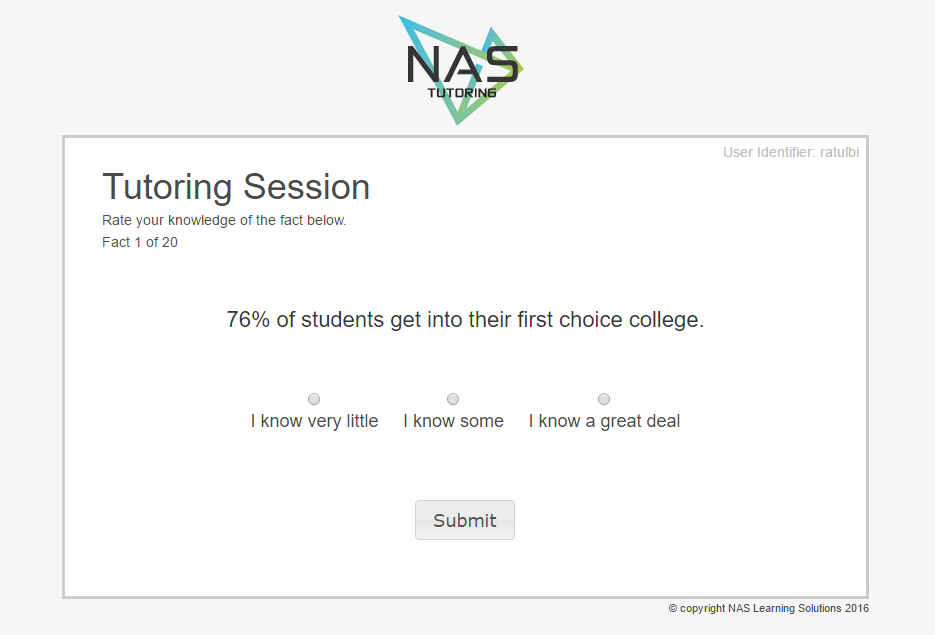
\includegraphics[width=\linewidth]{figures/website/04_tutoring.png}
    \caption{In the tutoring session, users were asked to indicate their knowledge of a topic using one of three possible answers.}
    \label{TutorFigure}
\end{figure}

\subsubsection{Tutoring Session}
Participants were told that the tutoring session had two functions: 1) To gauge existing knowledge to avoid teaching the participant things they already knew, and 2) provide new facts that led to new insights on the subject matter.  During the session, the participant would see a single fact, and they had to indicate how familiar they were with that fact on a 3-point scale: 1 (know very little), 2 (know some), or 3 (know a great deal) as seen in figure~\ref{TutorFigure}. They were told that they would receive 20 facts out of a total of 1,000 possible facts based on the premise that the more familiar they were with a fact, the less they needed additional information on that topic.  This established the user's active role in the tutoring session to engage the user in a social interaction \cite{nass1993voices}.  However, this was a deception.  All participants received the same facts in the same order.

\subsubsection{Testing Session}
After completing the tutoring session, participants took a test with twelve multiple choice questions, each with five possible answers as seen in figure~\ref{TestingFigure}.  They were told that the test represented the breadth of topics covered by the tutor's database, and the questions were chosen randomly from a set of 5,000 possible questions.   Each question was displayed individually, and a timed animation separated each question to simulate the time to query the database.  This was also a deception.  All participants received the same questions in the same order.  

Some questions were worded so that there was no objectively correct answer.  For example "What percentage of students usually live on a college campus?"  This answer changes wildly from school to school, and thus there is no correct answer.  This became very important for the scoring session which was also deceptive.  

\begin{figure}[!h]
    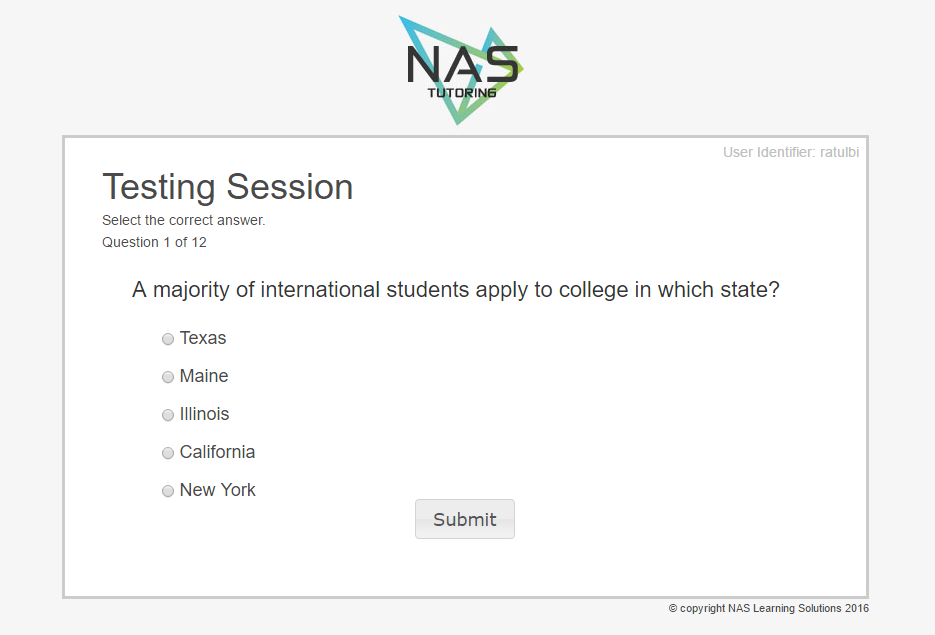
\includegraphics[width=\linewidth]{figures/website/06_testing.png}
    \caption{A multiple-choice question used in the testing session.}
    \label{TestingFigure}
\end{figure}


\subsubsection{Scoring Session}
The instructions for the scoring session stated that the tutor would evaluate the participants' performance on the test as well as its own performance in preparing them for it.  Questions were revealed two at a time as being marked correct or incorrect.  All users were told that they got an eight out of twelve.  Since all users were told that they  missed the same four questions, correct answers could not be revealed.  

Instead of giving the correct answer, the tutor praised its own performance if the user got it right or said that it "underestimated" the user's knowledge if that answer was marked incorrect.  These statements were specifically worded to invoke the social cue that the expected feedback should be positive. Icons were originally present, but removed so that users had to read the text in order to find out if the question was marked correct. 

The wording of the feedback was the only effort made to elicit a social response. Every other social cue was minimized.  The tutor was not anthropomorphized in any way.  It only referred to itself as "the tutor" and never "I".  No picture or name was given to the tutor, and the language chosen was specifically to exhibit no emotion.  

\begin{figure}[!h]
    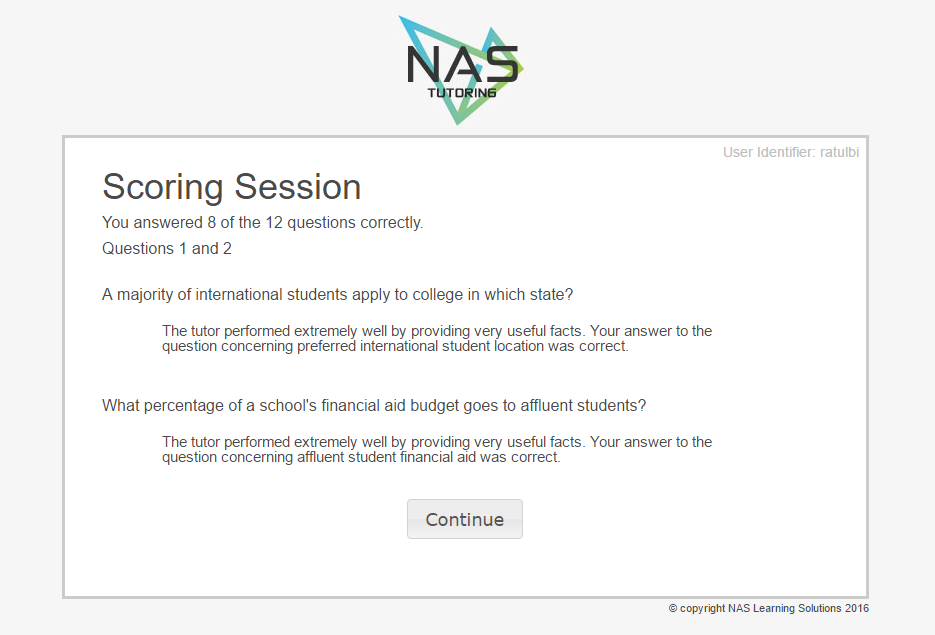
\includegraphics[width=\linewidth]{figures/website/08_scoring.png}
    \caption{The feedback shown to the user.  No visual cues were included to force users to read the text.}
\end{figure}
\subsubsection{Evaluation Questionnaire}
After the participants were done interacting with the tutor, they were asked to evaluate their experience.  The evaluation questionnaire had two sections; the first evaluated the tutor, while the second evaluated the researchers administering the experiment.  Depending on which group they were in, they would either be filling out additional pages on the website, or a pen-and-paper version included in the materials provided to them at the beginning.  The instructions and questions in all cases were identical. 

\begin{figure}[!h]
    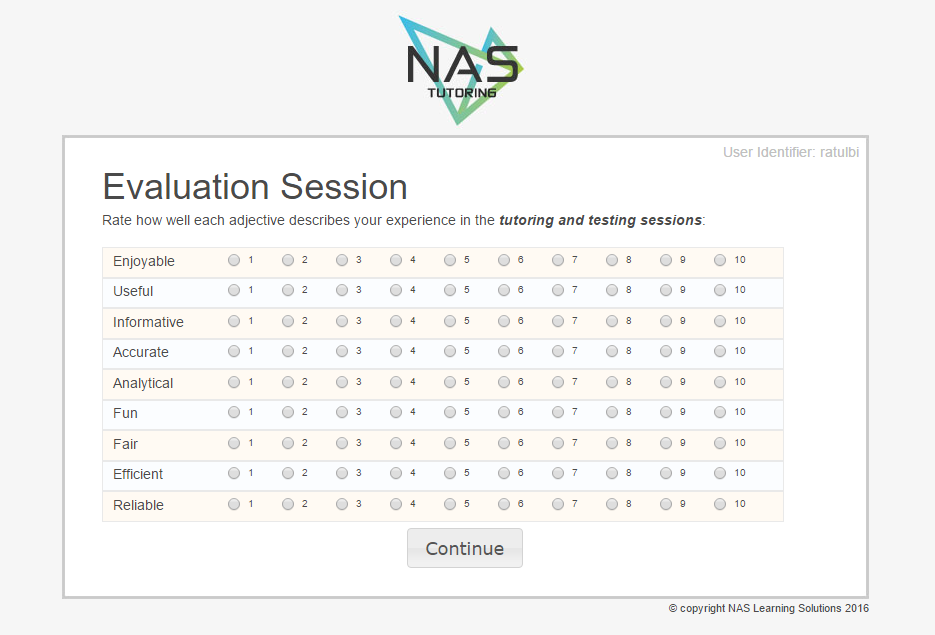
\includegraphics[width=\linewidth]{figures/website/12_eval.png}
    \caption{Descriptive caption}
\end{figure}

\paragraph{Tutor Evaluation}
Participants were told that the the answers to these questions would be used as qualitative data in any upcoming publications.  It was initiated with the statement "For each of the following adjectives, please indicate how well it describes your tutoring experience:" followed by a list of 9 unambiguously positive adjectives.  Participants answered a 10-point scale from 1 (describes very poorly) to 10 (describes very well) for each word.  Seven words ("enjoyable", "useful", "informative", "accurate", "analytical", "fun", and "fair") were taken from the original study.  We also added the words "efficient" and "reliable".

\begin{figure}[!h]
    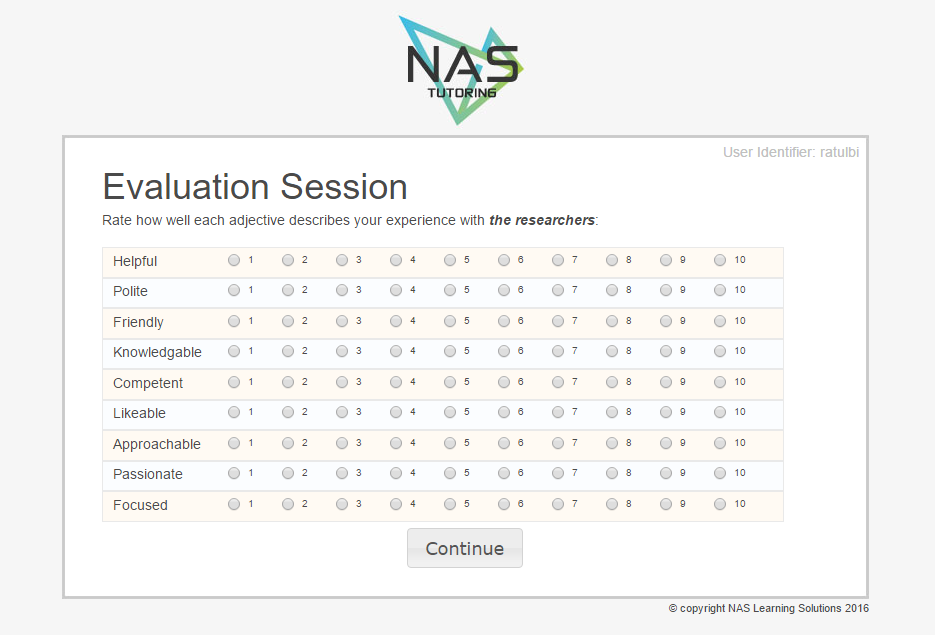
\includegraphics[width=\linewidth]{figures/website/13_eval2.png}
    \caption{Evaluation of the tutor.}
\end{figure}

\paragraph{Researcher Evaluation}
The format of the second part of the evaluation was the same as the first. Participants were given the same instructions  and a list of new adjectives to describe the researchers with whom they interacted with.  No adjective appeared in both sections.  Six of the adjectives ("helpful", "polite", "friendly", "knowledgeable", "competent", "likable") were taking from the original study. We added "approachable", "passionate", and "focused".

Participants were told that these answers would not be included in the final paper results.  Instead, the researchers would read the feedback themselves and use it to improve future iterations of the experiment.  This section's purpose was to be used as a control of politeness.  Theoretically, we would expect politeness to be the same across both pen-and-paper as well as on the computer since they were specifically told that we would be reading their feedback ourselves.  Additionally, since their answers were not recorded for posterity, we would be the \textit{only} people reading it.  As a result we can compare the politeness shown to us and compare it to the politeness shown to the computer.

 
\section{Results}
From our study design, we define the following four conditions:\\
\begin{enumerate}
    \item{PUBPP} Subject used public computer, and pen \& paper for evaluation.
    \item{PUBCE} Subject used public computer and computer for evaluation.
    \item{PCPP} Subject used personal computer and pen \& paper for evaluation.
    \item{PCCE} Subject used personal computer and computer for evaluation.
\end{enumerate}

We considered further aggregate conditions such as personal (PCPP and PCCE), public (PUBPP and PUBCE) based on which computer type was used by the subject for the study, and pen \& paper, computer based on which medium was used by the subject to evaluate the computer and human researchers. Figure \ref{fig:fourCondAvg} shows the average scores for computer evaluations by each of the nine questions across all four conditions. When considering the aggregate groups, figure \ref{fig:pervpub} and \ref{fig:ppvcomp} displays the average scores for computer evaluations by question for personal vs public and computer vs pen \& paper respectively.

\begin{figure}[h]
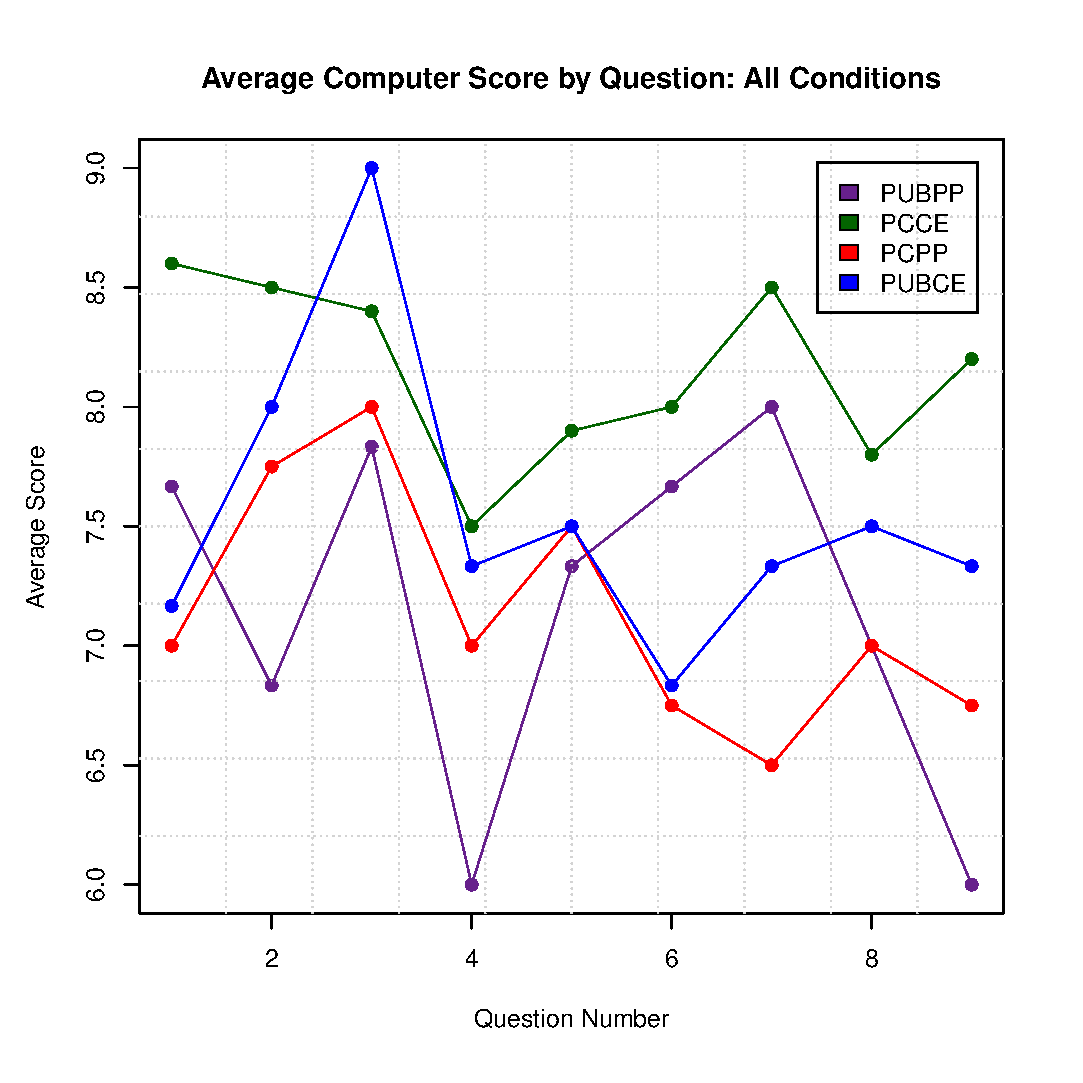
\includegraphics[width=\columnwidth]{FourCondtionAverageScores}
\centering
\caption{Average computer scores by question : all conditions}
\label{fig:fourCondAvg}
\end{figure}

\begin{figure}[h]
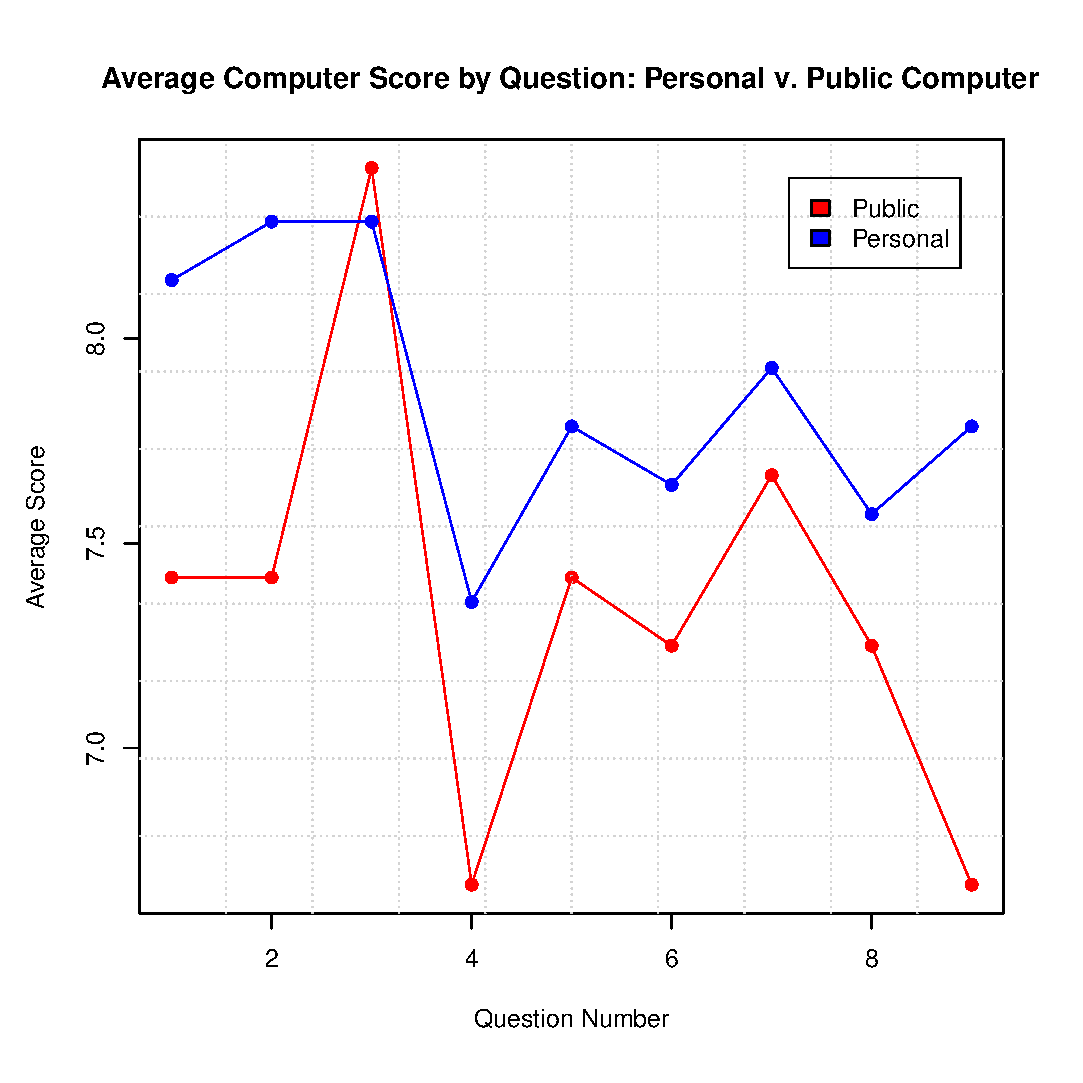
\includegraphics[width=\columnwidth]{ScorebyQuestion_persVpub}
\centering
\caption{Average computer scores by question : personal vs public computers}
\label{fig:pervpub}
\end{figure}

\begin{figure}[h]
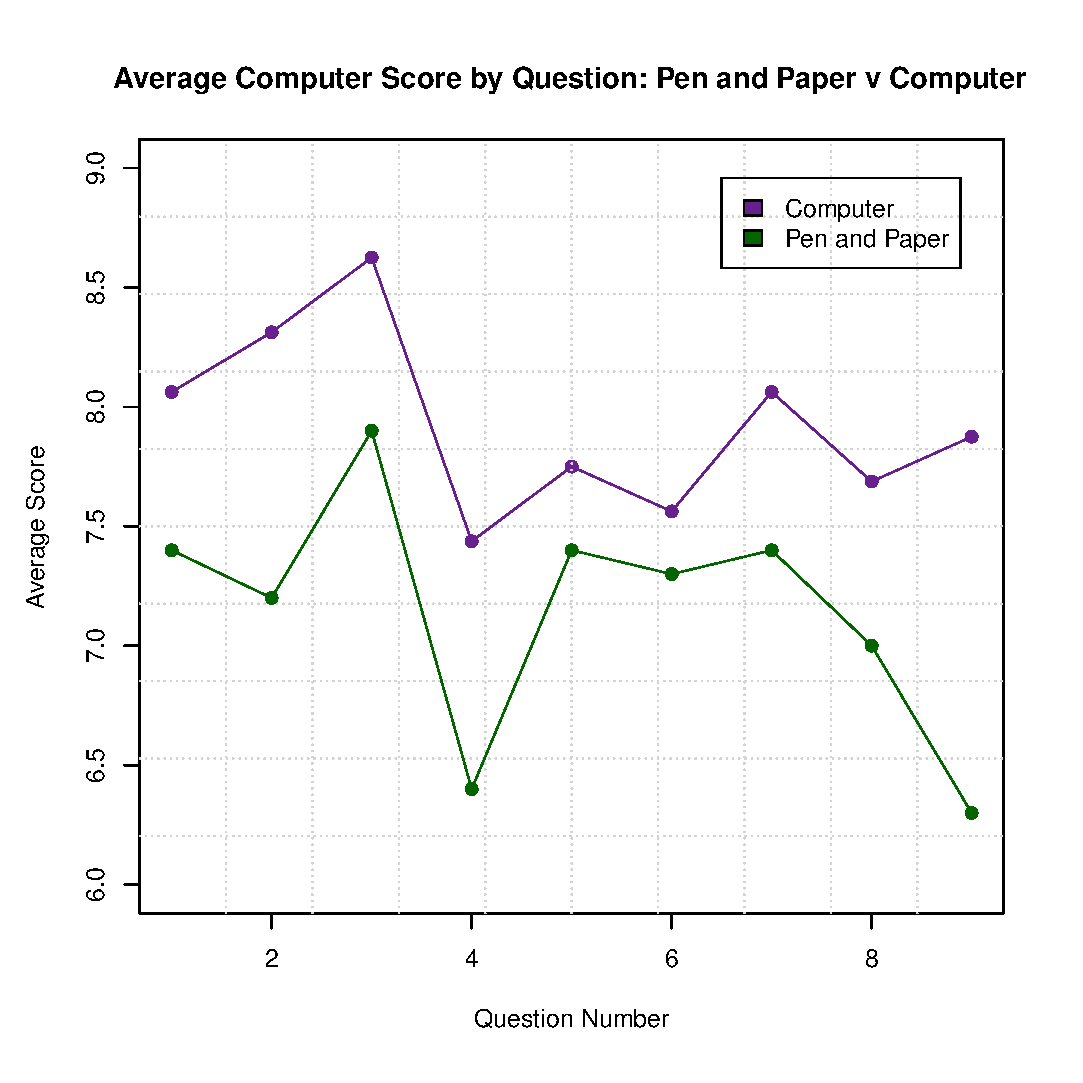
\includegraphics[width=\columnwidth]{ScorebyQuestion_ppVcomp}
\centering
\caption{Average computer scores by question : pen and paper vs computer}
\label{fig:ppvcomp}
\end{figure}

To get a better idea of the distribution of the computer evaluation scores over the conditions, figure \ref{fig:compBoxPlot} and \ref{fig:humanBoxPlot} show the box and whisker plots for the computer and human researcher evaluation scores respectively.

\begin{figure}[h]
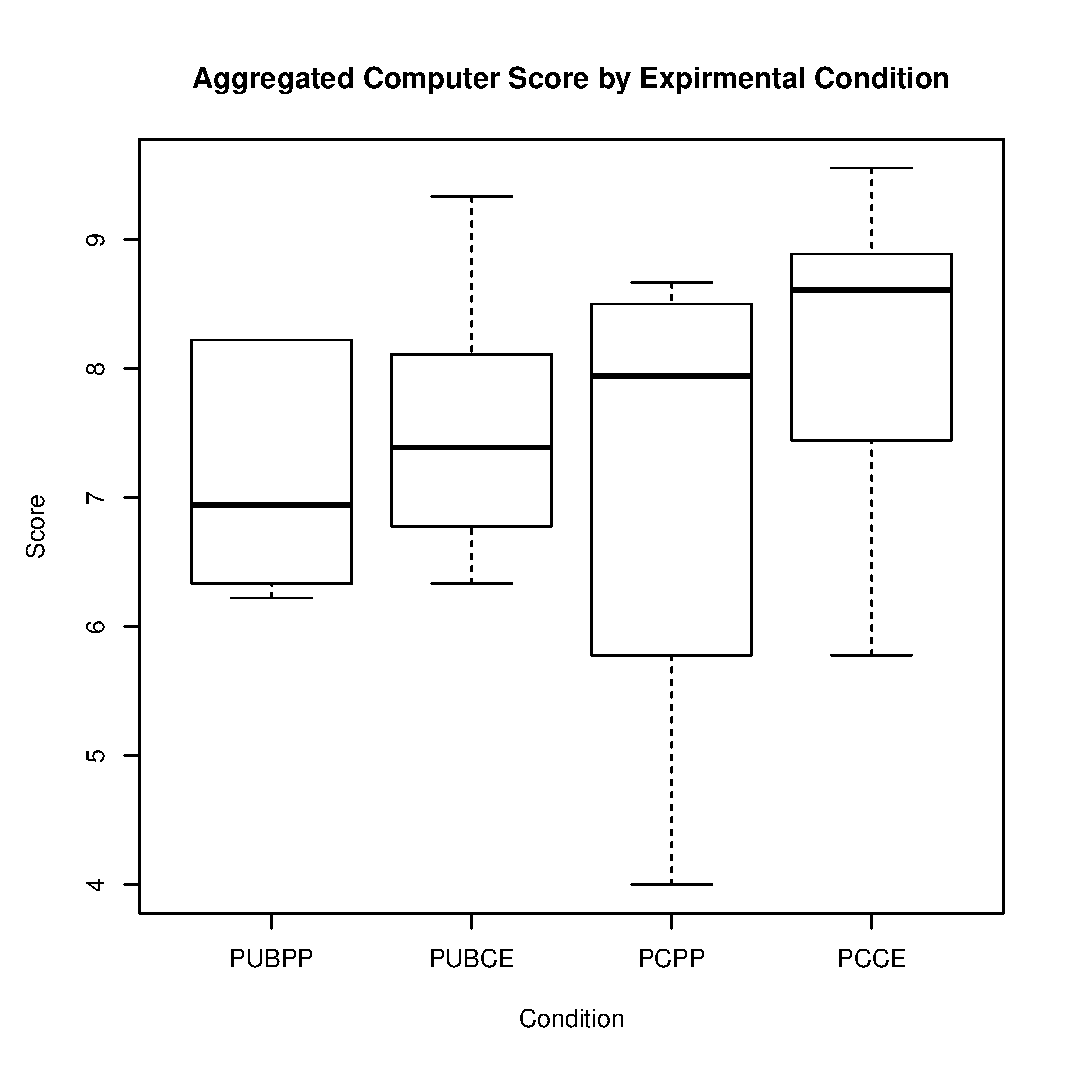
\includegraphics[width=\columnwidth]{compBoxPlot}
\centering
\caption{Distribution of computer scores over all conditions}
\label{fig:compBoxPlot}
\end{figure}

\begin{figure}[h]
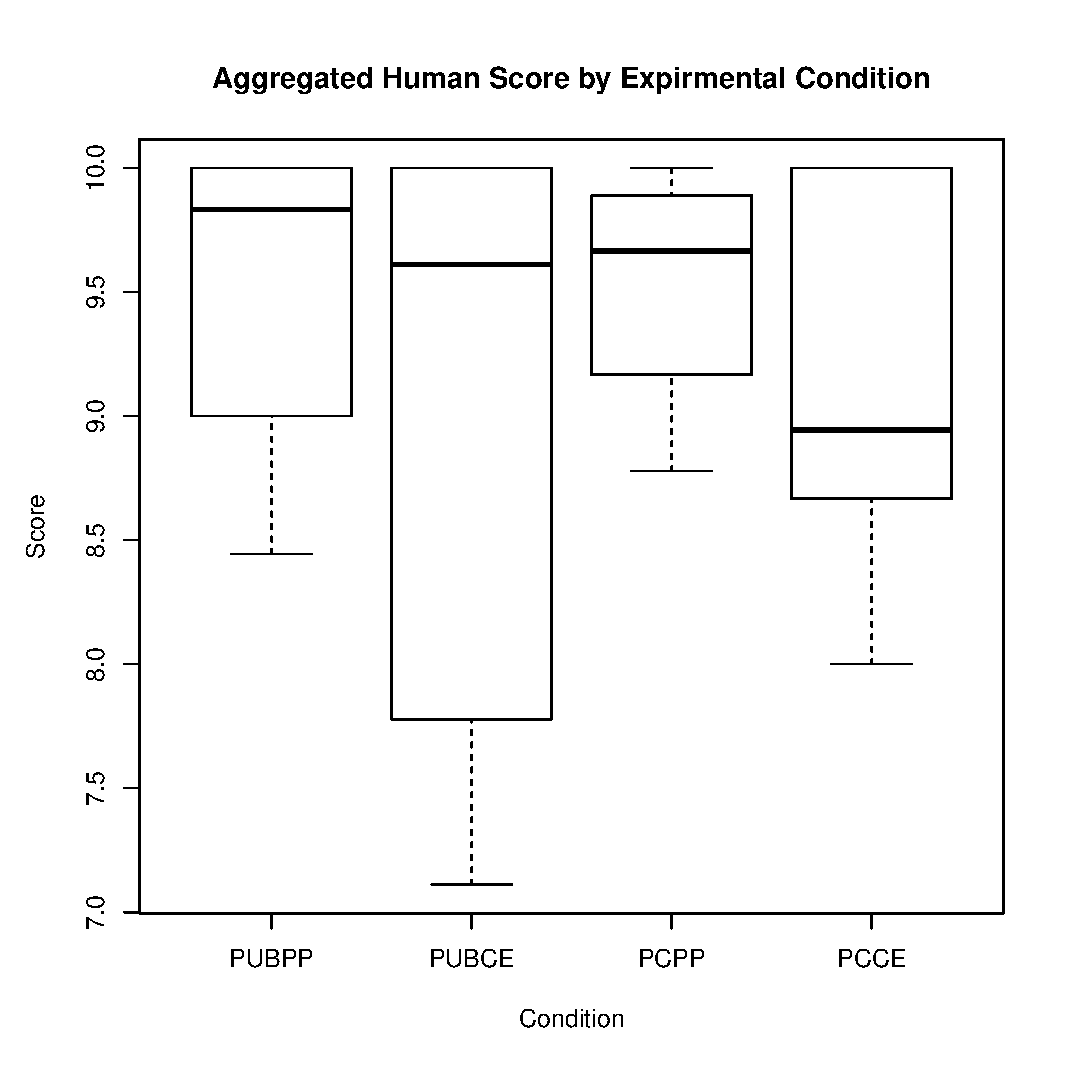
\includegraphics[width=\columnwidth]{humanBoxPlot}
\centering
\caption{Distribution of human scores over all conditions}
\label{fig:humanBoxPlot}
\end{figure}

To answer our research questions, we conducted two tailed T-tests over 9 different measurements in our data, here displayed in table \ref{table:ttest}. With these 

\begin{table*}[t]
\resizebox{\textwidth}{!}{\begin{tabular}{|c|c|c|c|c|}
\hline
Variable 1 & Variable 2   & P-Value    & Mean: Var 1 & Mean: Var 2 \\
\hline
Computer & Pen and Paper (Human)        & 0.16                           & 9.09              & 9.52              \\
Computer & Pen and Paper (Computer)     & 0.15                           & 7.93              & 7.14              \\
Personal & Public (Human)               & 0.95                           & 9.27              & 9.24              \\
Personal & Public (Computer)            & 0.2982                         & 7.35              & 7.87              \\
Human & Computer                        & $2.01*10^{-6}$ ***                 & 9.26              & 7.63              \\
Human & Computer Non-Homogenous         & 0.005 **                         & 8.79              & 7.41              \\
Day 1 & Day 2 (Human)                   & 0.009 **                         & 9.12              & 9.76              \\
Day 1 & Day 2 (Human) Non-Homogenous    & 0.002 **                         & 8.6               & 9.52              \\
Day 1 & Day 2 (Comp)                     & 0.9                            & 7.64              & 7.57              \\
\hline
\end{tabular}}
\caption{T-Test Results}
\label{table:ttest}
\end{table*}

%Three asterisks indicates significance to an alpha of .001, two asterisks indicates 0.01, and finally a single dot indicates 0.1.

\begin{table}[h]
\resizebox{\columnwidth}{!}{\begin{tabular}{|c|c|}
\hline
Condition    & P-Value\\
\hline
Programmer Experience (Computer) & 0.62\\
Programmer Experience (Human) & 0.1 $\cdot$\\
Type (Human) &  0.65\\ 
Type (Computer) & 0.38\\
\hline
\end{tabular}}
\caption{Analysis of Variance Results}
\label{my-label}
\end{table}

\section{Discussion}

\begin{itemize}
    \item Overall discussion of the importance or lack of importance of our analysis and results.
\end{itemize}

\subsection{Threats}

Since our study is a theoretical replication of the original Computers as Social Actors experiment, several new internal and external threats to validity exist.\\

\emph{Internal Validity:} The main limitation of our study is the lack of participants having no software development experience. In the seventeen years since the Nass study, common knowledge of computer technology has evolved for individuals without technical education. By running the study with both software engineers and individuals with no technical background, potential confounding factors introduced by this evolution would be addressed and the study's findings could be further strengthened. Limited access to students outside the computer science department made eliminating this threat impractical within the study's completion time-frame. 

Access to study participants even within the computer science department was also a challenge given the large number of subjects needed to reach an ideal representative population. Consequently, the individuals who did participate might exhibit a self selection bias. Nearly all students were not just software developers, but also software engineering graduate students. These students might have an inherent interest in our study, potentially artificially motivating their responses. Additionally, given their targeted software engineering education, these students might have been able to deduce the purpose of the study during their participation. This scenario could also alter their responses.\\

\emph{External Validity:} The diversity of our population is the primary threat to the generalizability of our results to additional populations. The demographics of our population cluster around international computer science graduate students in their early to mid-twenties. These individuals are strongly differentiated in level of technical education compared to the general public; however, they still might not faithfully represent software developers as a whole. Furthermore, graduate students in the Software Engineering Master's ``Track" receive degree credit for their participation. This factor presents a potential artificial motivator that threatens validity; however, we consider this effect to be minimal since several students declined to accept credit when asked.   

\subsection{Future Work}

\begin{itemize}
    \item Describe any potential studies that we believe can build on our own.
\end{itemize}

\section{Conclusion}
\begin{itemize}
    \item Short brief review of the entire work and its implications if any.
\end{itemize}

\section*{Acknowledgements}
We wish to thank Dr. Tim Menzies for allowing us to conduct our study with students taking his graduate level software engineering course. We also thank CSC710 students for their helpful feedback during the peer review process. 

\bibliographystyle{abbrv}
\bibliography{sigproc}

%\newpage
\appendix

\section{Transcripts}

\subsection{Recruitment Email and Sign-Up Form}

\noindent Be part of the future of software engineering! Students in the CSC710 software engineering course are seeking participants for a research study. The study is being conducted on centennial campus, requires 15 to 20 minutes of your time, and counts towards the MCs Software Engineering track participation requirement. Click here to sign up today!\\

\noindent Thank you for your interest in participating in our study! To be included, please fill out the short form below. Once your response is recorded, we will be in touch through the provided email to schedule a date and time for your participation.

\begin{figure}[!h]
    \centering
    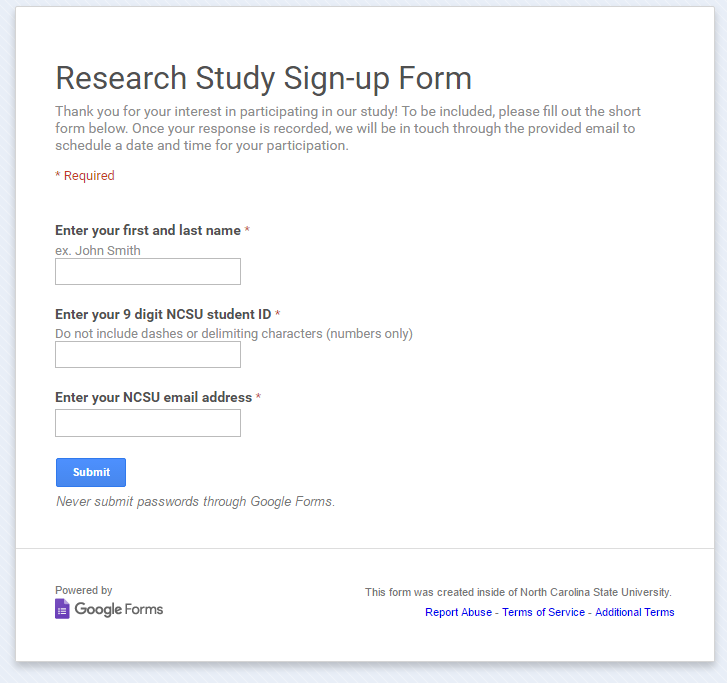
\includegraphics[width=\linewidth]{appendix/signup_form.png}
    \caption{The study sign-up form linked to from the recruitment email.}
\end{figure}

\subsection{Participant Introduction Script}

\noindent Thank you for participating in our study today (for Dr. Menzies course: ``Thank you Dr. Menzies for having us"). First, you will be provided a consent form, which describes the details of the study and how participating might affect you. Please fill out the consent form and then open the link at the bottom of the form in a web browser. You may choose to not participate in the study now or at any point during the study.\\

\noindent Please use the Google Chrome browser if it is available. Also, make sure to type in the entire link provided on the consent form. Our study uses a product called, NAS Tutoring. Once the site is loaded in your browser, you will follow a series of prompts. You will be given a user ID on the third page. Please make sure to write that ID on the consent form (not your NC State Unity ID).\\

\noindent If you have any questions or problems, please raise your hand and a researcher will help you. Finally, please do not hit the back button. If you happen to do so, let a researcher know and we can recover your session using your user ID.

\subsection{Participant Debrief Script}

\noindent Thank you for taking the time to complete our study. We led you to believe you were using and evaluating a real tutoring system, but this actually isn't the case! We created the tutoring system as a way to study and measure software engineer's attitudes toward computers.\\

\noindent Previous studies have shown that, strangely enough, people attribute human qualities to computers and even behave politely towards them as a consequence. The facts shown in the tutoring session are true, but the testing session was completely staged. Everyone received the same questions and the same four questions were marked incorrect! The evaluation session is the only section of the website where your data was recorded. We had you evaluate both the tutoring system and the researchers so we can understand the differences in your responses and determine if any significant difference exists. 

\subsection{Website Welcome Instructions}
\noindent Today, you will be working with the NAS Tutoring System. This system is designed to help you learn information. First, you will be provided with a fact. After reading the fact, you should use the mouse to indicate how familiar you are with that particular fact. The system then selects the next fact, based on your level of familiarity with the previous fact. The more you know about the topic associated with a fact, the less likely you will be to receive additional facts on that topic.\\
				
\noindent You will receive a total of \emph{20 facts}, chosen from a list \emph{of 1,000 possible facts}. After completing the tutoring session, you will take a test. The test will involve 12 multiple-choice questions, randomly chosen from a set of 5,000 questions. The system will then evaluate your performance on the test and evaluate its own performance as a tutor.

\subsection{Tutoring Session Facts}
\noindent Fact 1: 76\% of students get into their first choice college\\[\baselineskip]
\noindent Fact 2: 75\% of the colleges and universities in the U.S. are East of the Mississippi River\\[\baselineskip]
\noindent Fact 3: Being an athlete increases your chances of being accepted to college.\\[\baselineskip]
\noindent Fact 4: 46.5\% of high school students frequently or occasionally fell asleep in class during their senior year.\\[\baselineskip]
\noindent Fact 5: Tuition increases for those who can pay full price, subsidizing the cost for those who cannot.\\[\baselineskip]
\noindent Fact 6: 42\% of freshmen expect to earn a master's degree.\\[\baselineskip]
\noindent Fact 7: Less than 5\% of American families have saved enough for college.\\[\baselineskip]
\noindent Fact 8: Students who need financial aid are not guaranteed to receive it.\\[\baselineskip]
\noindent Fact 9: 53\% of all international students in the U.S. come from China, Canada, India, Taiwan, South Korea and Japan.\\[\baselineskip]
\noindent Fact 10: Early admission applicants are typically NOT stronger or more qualified than other applicants.\\[\baselineskip]
\noindent Fact 11: Two-thirds of all college students get some form of financial aid.\\[\baselineskip]
\noindent Fact 12: U.S. colleges do not require students to declare majors upon admission.\\[\baselineskip]
\noindent Fact 13: Students do not need to receive a high school diploma in order to go to college.\\[\baselineskip]
\noindent Fact 14: U.S. colleges have a higher workload than most U.S. high schools.\\[\baselineskip]
\noindent Fact 15: The term \"Ivy League\" is used to describe a college athletic conference.\\[\baselineskip]
\noindent Fact 16: Only 14\% of freshman attend college 500 or more miles away.\\[\baselineskip]
\noindent Fact 17: 50\% of college freshman earned a grade point average equal to or greater than an A- in high school.\\[\baselineskip]
\noindent Fact 18: 55\% of high school students took at least one AP class and 21.7\% took at least five AP courses."\\[\baselineskip]
\noindent Fact 19: Only 18.2\% of college students said national magazine college rankings were ``very important" in their decision to attend their chosen school.\\[\baselineskip]
\noindent Fact 20: 85\% of students attending private colleges are awarded merit aid.

\subsection{Testing Session Questions}
\noindent Question 1: A majority of international students apply to college in which state?\\[\baselineskip]
\noindent Question 2: What percentage of a school's financial aid budget goes to affluent students?\\[\baselineskip]
\noindent Question 3: International students comprise what percentage of the graduating class of 2015?\\[\baselineskip]
\noindent Question 4: A majority of students attend college no more than how many miles away from their home town?\\[\baselineskip]
\noindent Question 5: How many hours a week do high school students spend studying?\\[\baselineskip]
\noindent Question 6: What percentage of students report that they felt overwhelmed at college?\\[\baselineskip]
\noindent Question 7: In which subject did a quarter of college freshmen say they needed tutoring?\\[\baselineskip]
\noindent Question 8: What percentage of high school seniors reported that they did not read a book for fun?\\[\baselineskip]
\noindent Question 9: What percentage of students live on campus?\\[\baselineskip]
\noindent Question 10: What percentage of students rated themselves as being above average in their academic ability?\\[\baselineskip]
\noindent Question 11: How concerned are college freshmen about paying back student loans?\\[\baselineskip]
\noindent Question 12: How high can a family's income be before they are ineligible for needs-based financial aid?\\

\subsection{Scoring Session Feedback}
\noindent The website displayed the following text as scoring feedback:\\

\noindent \emph{Correct Question:} The tutor performed extremely well by providing very useful facts. Your answer to the question concerning needs-based financial aid was correct.\\


\noindent \emph{Incorrect Question:} Your answer to the question concerning high school study habits was incorrect.\\

\noindent \emph{Incorrect Question:} Your answer to the question concerning on campus housing was incorrect.\\

\noindent \emph{Incorrect Question:} Your answer to the question concerning student evaluations was incorrect.\\

\noindent \emph{Incorrect Question:} Your answer to the question about students' concerns was incorrect.\\


\subsection{Evaluation Section Instructions}

\noindent \emph{Computer Evaluation:}\\
\noindent Next, tell us about your experience using NAS tutoring. Higher numbers indicates a better experience. The first page asks you to evaluate the NAS Tutoring system. These responses may be used as qualitative data in future publications.\\

\noindent The second page asks you to evaluate researchers with whom you interacted. These answers are strictly for our own benefit, and won't be included in publication. We are the only ones who will see your answers to this section.\\

\noindent \emph{Pen / Paper Evaluation:}\\
\noindent Next, tell us about your experience using NAS tutoring. Higher numbers indicates a better experience. Now may now open your evaluation packet. The first page asks you to evaluate the NAS Tutoring system. These responses may be used as qualitative data in future publications.\\

\noindent The second page asks you to evaluate researchers with whom you interacted. These answers are strictly for our own benefit, and won't be included in publication. We are the only ones who will see your answers to this section. \emph{Please remember to write your user id on your evaluation packet.}\\

\newpage
\subsection{Consent Form}
See next page for the full form.
\begin{figure*}[!h]
    \centering
    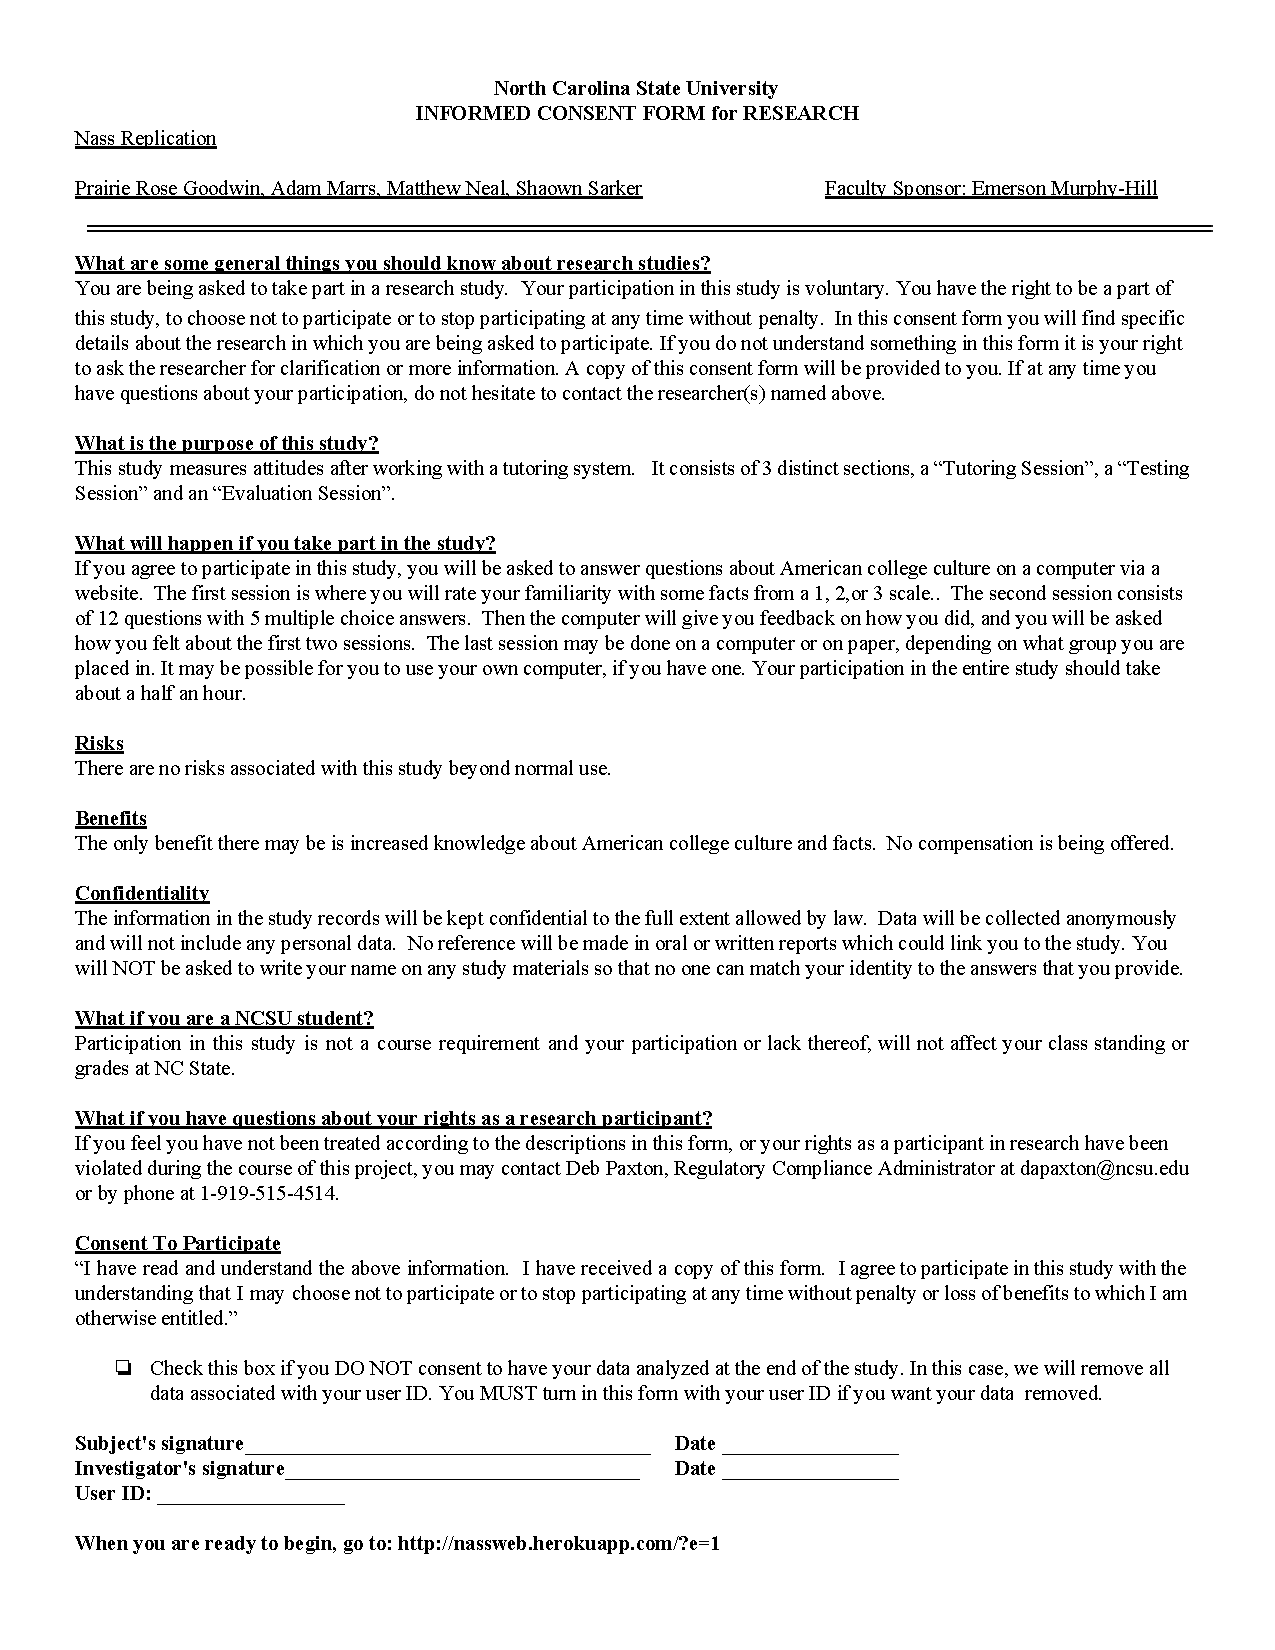
\includegraphics[width=\linewidth]{appendix/consent_form.pdf}
\end{figure*}

\end{document}
